\documentclass[a4,12pt]{article}

\usepackage[francais]{babel}
\usepackage[utf8]{inputenc}
\usepackage[T1]{fontenc}
\usepackage[babel=true]{csquotes}
\usepackage{amsmath}
\usepackage{amssymb}
\usepackage{float}
\usepackage{graphicx}
\usepackage{wrapfig}
\usepackage{hyperref}
\usepackage{array,multirow,makecell}
\usepackage[
backend=biber,
style=alphabetic,
sorting=ynt
]{biblatex}

\addbibresource{biblio.bib}
\frenchbsetup{StandardLists=true}
\usepackage{enumitem}
\setlength\parindent{20pt}
\begin{document}
\begin{titlepage}
\title{ Documentation technique sur la classe Math.}
\author{Fischman Adrien, Geoffroy Germain.}
\date{}

\maketitle

\rule[0.5ex]{\textwidth}{0.2mm}
Ce document a pour but d'expliquer la conception de la classe Math.decah.\\
Il présente à la fois les algorithmes utilisés, ainsi que les choix mathématiques et informatiques nécessaires à l'implémentation, mais aussi la démarche qui a permis d'aboutir.\\
La validation et les limites de nos algorithmes sont décrites au fur et à mesure, expliquant les choix que nous avons étés amenés a prendre.

\rule[0.5ex]{\textwidth}{0.2mm}

\end{titlepage}
\tableofcontents
\newpage
\section{Introduction.}
La classe Math contient différentes méthodes :
\begin{itemize}
    \item float ulp(float f)
    \item float sin(float f)
    \item float cos(float f)
    \item float asin(float f)
    \item float atan(float f)
\end{itemize}
L'implémentation de ces différentes méthodes se doit donc de minimiser les sources d'imprécisions, qui proviennent d'une part des approximations mathématiques nécessaires aux algorithmes utilisés mais aussi des limites de précision liées à la représentation des nombres flottants simple précision, afin d'atteindre la meilleur approximation possible des ces différentes fonctions mathématiques.\\
On notera que tous les angles utilisés et donc les arguments des fonctions sin et cos sont exprimés en radian.\\
\subsection{Nombre flottant simple précision.}
La représentation des nombres flottants simple précision se fait en un mot de longueur 32 bits avec : un bit de signe, 8 bits pour l'exposant et 23 bits pour la mantisse.\\
Un nombre flottant normalisé (ie dont l'exposant décalé est différent de 0 et de 127 et que le bit de poids fort de la mantisse est 1) est de valeur $x$ est donné par : \\
$$ x = s.2^{e}.m\ ,\ avec
 \left \{
    \begin{array}{l}
    s = \pm 1\ repr\acute esente\ le\ signe (selon\ le\ bit\ de\ signe)\\
    e\ est\ l'exposant\ avant\ son\ d\acute ecalage\ de\ 127\\
    m = 1 + mantisse,\ repr\acute esente\ la\ partie\ significative\ (en\ binaire)\\
    \end{array}
\right.
$$
\begin{figure}[b]
    \centering
    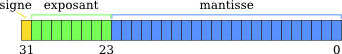
\includegraphics{float.png}
    \caption{Nombres flottants simple précision.}
    \label{Représentation des nombres flottants simple précision.}
\end{figure}

\subsection{Mesure de l'approximation.}
Afin de mesurer l'approximation faite par nos calculs, nous utilisons l'unité de précision élémentaire sur les nombres flottants : ULP (Unit in the Last Place). L'ULP d'une flottant f représente la distance en nombre flottant entre f et le flottant le plus proche de f.\\
Ainsi la précision des calculs se mesure en ulp. Lorsque que l'on approche un nombre $x$ par le nombre approximé $\tilde x$, on mesure $ \frac{|x - \tilde x|}{ulp(x)} $ pour exprimer l'écart en ulp entre la valeur approchée et la valeur exacte.

\subsection{Validation des algorithmes.}
Pour confronter nos résultats avec les valeurs mathématiques attendues, nous utilisons les fonctions prédéfinies de Java. On compare alors nos valeurs à celle retournée par Java ce qui implique donc que la validation de nos résultats ne constitue qu'une seconde approximation de la valeur mathématique.\\
Cependant, en pratique, atteindre un niveau de précision de quelques ulp est suffisant pour notre implémentation et c'est l'objectif que nous nous sommes fixé.
\section{Fonction ulp.}
\subsection{Implémentation.}
La fonction ulp mesure la distance entre deux flottants, en particulier $ulp(f)$ représente la distance entre $f$ et le flottant supérieur le plus proche $\tilde f$.
L'implémentation de la fonction ulp a nécessité, avant tout, celle d'une fonction puissance : \textbf{ float Math.\_power(float x, int y)}. \\
La méthode ulp a pour but de calculer l'exposant de son argument $f$, représenté en flottant simple précision, puis de retourner $ulp(f)$ en calculant la distance entre $f$ et $\tilde f$ où $\tilde f$ à la même représentation binaire que $f$ à la différence du premier bit de la mantisse qui diffère, c'est donc le flottant le plus proche de $f$.\\
Pour l'implémentation de la méthode ulp, nous avons utilisé la parité de la fontion ulp pour se ramener au cas d'un argument positif. De plus, en langage deca, on ne peut pas prendre en compte les valeurs NaN et les différents infinis comme en Java, on peut tout de même renvoyer des valeurs particulières pour les arguments $ MAX\_VALUE ( = 2^{127}) $ et $ MIN\_VALUE ( = 2^{-149}) $ qui correspondent respectivement aux valeurs maximum et minimum qu'un flottant peut prendre en représentation simple précision. Nous avons choisi de rester fidèle à l'implémentation faite en Java et nous avons respecté les mêmes spécificitées : 
$$
 \left \{
    \begin{array}{l}
        ulp(MAX\_VALUE) = ulp(MIN\_VALUE) = 2^{104} \\
        ulp(0) = MIN\_VALUE 
    \end{array}
\right .
$$
\subsection{Validation.}
Les résultats obtenus pour l'implémentation de la fonction ulp sont excellents puisque le résultat obtenu est celui de la méthode Math.ulp(float f) de Java, et ceci pour n'importe quel nombre.\\
\\

\hspace{-3cm}
\begin{tabular}{|c|c|c|c|c|c|}

\hline 
 & intervalle & nombre d'erreur($ >= 1 ulp$) & erreur max(ulp) & pas & nombres de tests \\
\hline 
ulp & $[0;10\ 000]$ & 0 & $0$ & $2^{-10}$ & 10 240 000\\
\hline
ulp & $[ 1\ 000\ 000 ;1\ 010\ 000]$ & 0 & $0$ & $2^{-4}$ & 160 000\\
\hline
\end{tabular}

\section{Fonction sin et cos.}
\subsection{Démarche d'implémentation.}
L'implémentation des fonctions sinus et cosinus a nécessité quelques ajustements. Nous avons commencé par utiliser l'algorithme de Cordic, puis finalement nous avons continué en utilisant le développement en série entière des ces fonctions pour gagner en précision. \\
La difficulté de l'utilisation des développements en série entière réside en la réduction des arguments d'entrés, pour cela nous avons dû implémenté l'algorithme de réduction de Cody \& Waite.
\subsubsection{Algorithme de Cordic \footnote{Wikipédia : https://fr.wikipedia.org/wiki/CORDIC}.}
L'algorithme de Cordic consiste à calculer $tan(\theta)$ en appliquant au vecteur de coordonnée (x,y) une suite de rotations d'angles décroissants tendant vers 0 et dont la somme est égale à $\theta$. Le quotient $\frac{y}{x}$ est alors une approximation de $tan(\theta)$. \\
Ainsi, on peut retrouver les valeurs des sinus et des cosinus en utilisant les relations : 
$$
 \left \{
    \begin{array}{l}
        tan(\theta) = \frac{sin(\theta)}{cos(\theta)}\ \\
        cos(t) = \frac{1-t^2}{1+t^2}\ avec\ t = tan(\frac{\theta}{2})
    \end{array}
\right .
$$
Dès lors, nous avons implémenté\footnote{http://www.trigofacile.com/maths/trigo/calcul/cordic/cordic.htm#haut} une fonction racine carrée : \textbf{float Math.\_sqrt(float x)}. Cette fonction fait une recherche dichotomique sur les flottants inférieurs $\tilde x$ à $x$ qui vérifie $ \tilde x^2 = x $. Cependant, les résultats de l'algorithme de Cordic n'étaient pas convaincant, en effet on atteingnant des erreurs moyennes d'une trentaine d'ulp. \\
\\

\hspace{-4cm}
\begin{tabular}{|c|c|c|c|c|c|c|}

\hline 
 & intervalle & nb erreur($ >1 ulp$) & erreur max(ulp) & erreur moyenne(ulp) & pas & nombres de tests \\
\hline 
cosCordic & $[0; 2\pi]$ & 324 031 & $1\ 153\ 000$  & $31.9$ & $2^{-17}$ & 823 550 \\
\hline
\end{tabular}

\subsubsection{Développement en série entière.}
Pour le calcul de $cos$ et $sinus$ nous avons utilisé les formules classiques du développement en série entière de ces fonctions:
\begin{equation}
\sin x=\sum_{n=0}^{+{\infty}}(-1)^n\,{\frac{x^{2n+1}}{(2\,n+1)!}}
\end{equation}
\begin{equation}
 \cos x=\sum_{n=0}^{+{\infty}}(-1)^n\,{\frac{x^{2n}}{(2\,n)!}}
\end{equation}
Nous remarquons que le coefficient i du $cos$ dépend du coefficient i-1:\\
$$a_{2i} =\frac{-a_{2(i-1)}}{(2i-1)2i}$$\\
Nous remarquons que le coefficient i du $sin$ dépend du coefficient i-1:\\
$$a_{2i+1} =\frac{-a_{2i-1}}{(2i+1)2i}$$\\
Cette méthode nous évite des calculs coûteux de calcul de factorielles.
Nous utilisons un critère d'arrêt pour le calcul de ces fonctions:On ajoute un terme à la somme partielle tant que celui ci à du sens, c'est à dire tant que ce terme est supérieur à l'ulp de la somme partielle.
Ce critère d'arrêt permet d'éviter de calculer des termes non nécessaires car l'ordre à laquelle il faut s'arrêter dépend de la valeur de x.\\
\\

Toutefois, l'implémentation en utilisant une simple réduction d'argument n'était pas suffisante pour atteindre une précision de seulement quelques ulp. C'est pourquoi nous avons eu recours à l'algorithme de Cody \& Waite.\\
\\

\hspace{-2cm}\begin{tabular}{|c|c|c|c|c|c|}

\hline 
 & intervalle & nombre d'erreur($ > 1 ulp$) & erreur max(ulp) & pas & nombres de tests \\
\hline 
sin & $[0;\pi /4]$ & 229 & $2$ & $2^{-17}$ & 102944\\
\hline
sin & $[\pi /4;\pi /2]$ & 985 & $3$ & $2^{-17}$ & 102944\\
\hline
sin & $[\pi /2;\pi .3/2]$ & 5761 & $3$ & $2^{-17}$ & 411775\\
\hline
\end{tabular}\\
\\

\hspace{-2cm}\begin{tabular}{|c|c|c|c|c|c|}

\hline 
 & intervalle & nombre d'erreur($ >  ulp$) & erreur max(ulp) & pas & nombres de tests \\
\hline
cos & $[0;\pi /8]$ & 3(>1ulp) & $2$ & $2^{-17}$ & 51472\\
\hline
cos & $[\pi /8;\pi /4]$ & 4544(>1ulp) & $2$ & $2^{-20}$ & 411775\\
\hline
cos & $[\pi /4;3\pi /8]$ & 5771(>1ulp) & $2$ & $2^{-20}$ & 411775\\
\hline
cos & $[3\pi /8;\pi /2]$ & 2166(>1ulp) & $2$ & $2^{-20}$ & 411775\\
\hline
cos & $[\pi /2;\pi .1.005/2]$ & 1025(>50ulp) & $1.2303662E7$ & $2^{-17}$ & 1030\\
\hline
cos & $[\pi /2;5\pi /8]$ & 316165 & 279598 & $2^{-20}$ & 411775\\
\hline
\end{tabular}


\subsubsection{Algorithme de Cody \& Waite\footnote{Jean-Michel Muller, Elementary Functions, Algorithms and Implementation, second edition, pages 177--184, 2005}.}
L'algorithme de Cody \& Waite est une méthode de réduction additive d'un argument $x$ sur un intervalle $[-C ; C]$.
Dans notre cas, $C = \pi /4$ et $x$ correspond à l'argument des fonctions sinus ou cosinus. On cherche donc à exprimer : 
$ cos(\tilde x) \ avec \ \tilde x = x - k.C $. \\
La méthode de Cody \& Waite suggère de découper en deux valeurs $C_{1}$ et $C_{2}$ de façon à ce que : 
\begin{itemize}
    \item $C_{1}$ soit très proche de $C$
    \item $C =C_{1} + C_{2} $
\end{itemize}
Ainsi, plutôt que de calculer $ x -k.C $, on calcule dorénavant : $ (x - k.C_{1}) - k.C_{2} $ \\
Ceci a pour conséquence d'évaluer des nombres flottants comparables et donc de bénéficier de la précision de $C_{1} + C_{2}$ 
plutôt qu'uniquement celle de $C$.\\
\\
En pratique, nous avons découper notre constante $C = \pi /4$ en $16$ constantes en récupérant la valeur de $\pi$ en binaire sur 64 bits, puis en découpant par tranche de 4 bits pour obtenir les 16 différentes valeurs.\\
Ainsi, on se ramène à l'intervalle $[-\pi /8 ; \pi / 8]$ et en fonction de la valeur de $k\ modulo\ 8$ on récupère la valeur du sinus ou du cosinus en utilisant les résultats : $$ sin( a + b ) = cos(a)sin(b) + sin(a)cos(b) \ et \ cos(a + b) = cos(a)cos(b) - sin(a)sin(b) $$


\subsection{Validation.}
La méthode sin donne une approximation à 5 ulp d'écart au maximum.\\
Pour des petits angles ($<\pi /8$), la précision est de 1 ulp dans le pire cas.\\
\\

\hspace{-4cm}\begin{tabular}{|c|c|c|c|c|c|c|}

\hline 
 & intervalle & nb erreur($>1 ulp$) & erreur max(ulp)& erreur moyenne(ulp) & pas & nb tests \\
\hline 
sin & $[0; \pi /8]$             & 0       & $1$ & null        &$2^{-23}$ & 3 294 199\\
\hline 
sin & $[\pi /8; 2\pi]$          & 1117838 & $5$ &$2.13$ & $2^{-20}$ & 6 176 623\\
\hline 
sin & $[1\ 000; 1\ 000 + 2\pi]$     & 17777    & $5$ &$2.13$ & $2^{-14}$ & 102 944\\
\hline 
sin & $[100\ 000; 100\ 000 + 2\pi]$ & 127      & $4$ &$ 2.20$ & $2^{-7}$ & 804\\
\hline
\end{tabular}
\newline
\begin{figure}[h!]
    \hspace{-5cm}
    \centering
    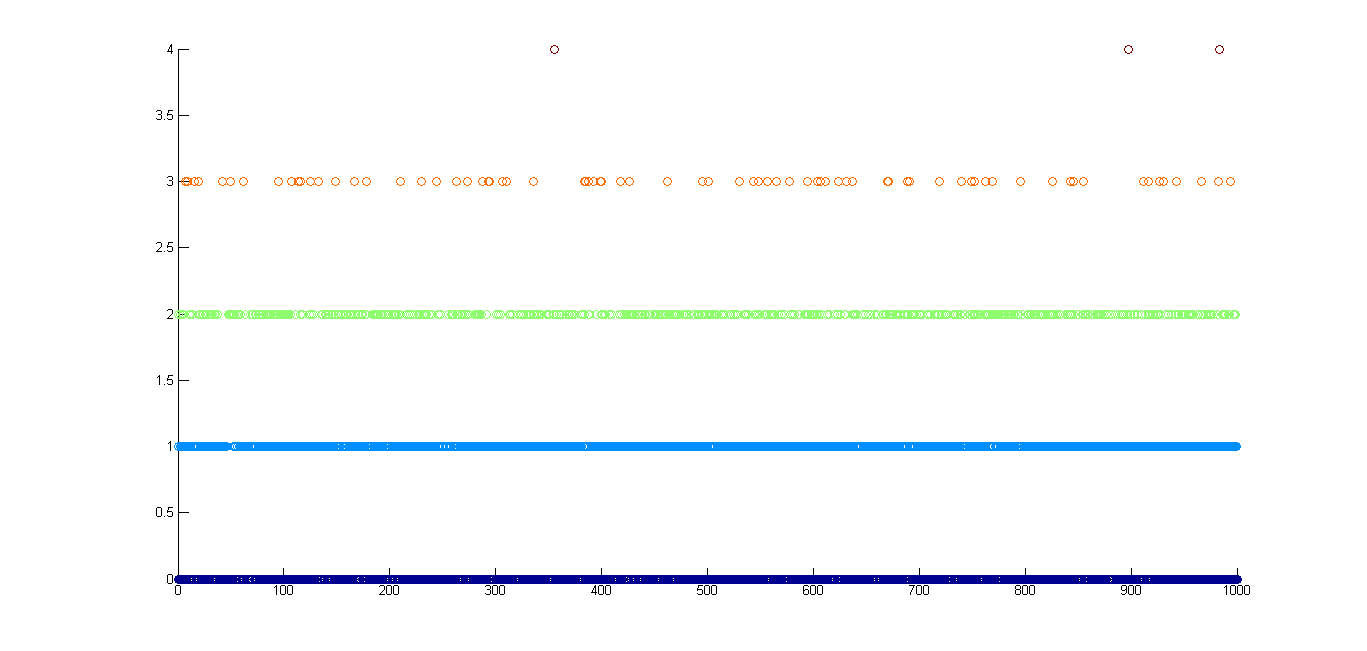
\includegraphics[scale=0.5]{sin1000}
    \caption{Nombre d'ulp d'erreur en fonction de x, pour sin(x)}
    \label{fig:my_label}
\end{figure}
\newline
\begin{figure}[h!]
    \centering
    \hspace{-5cm}
    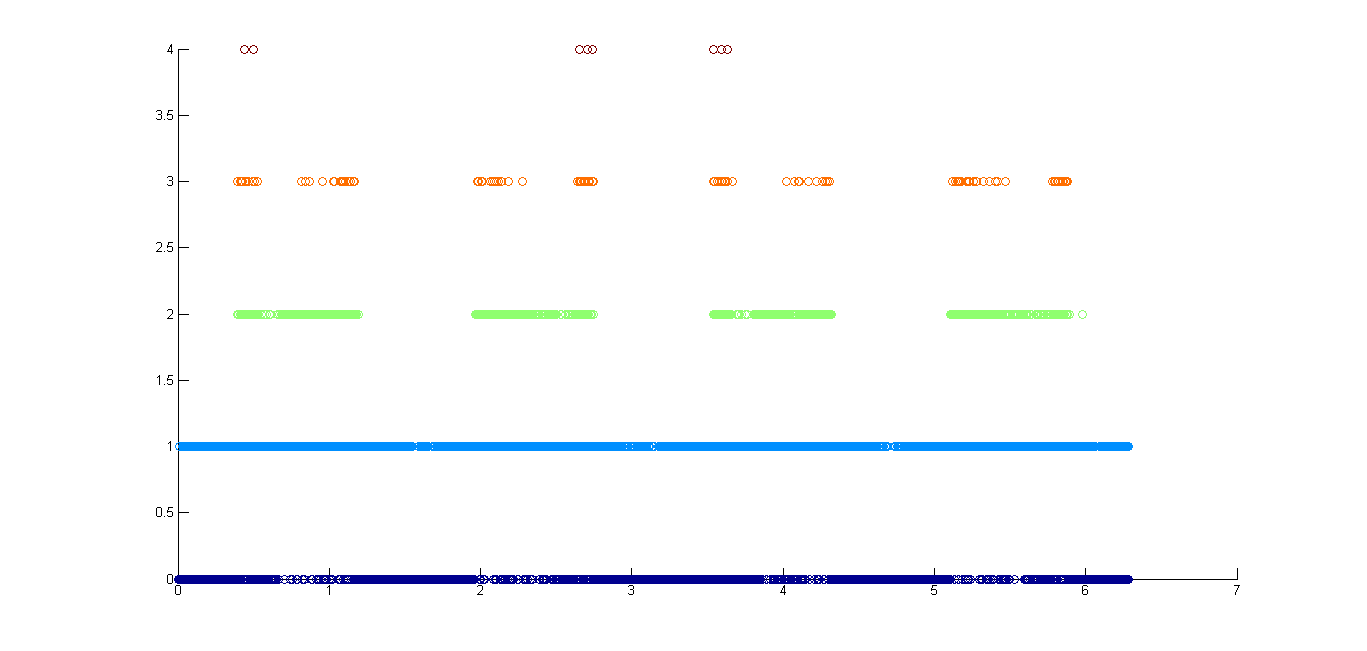
\includegraphics[scale=0.5]{sin2PI}
    \caption{Nombre d'ulp d'erreur en fonction de x, pour sin(x)}
    \label{fig:my_label}
\end{figure}
\\
\clearpage
La méthode cos donne une approximation à 6 ulp d'écart au maximum.\\
Pour des petits angles ($<\pi /8$), la précision est de 2 ulp dans le pire cas.\\
\\

\hspace{-4cm}\begin{tabular}{|c|c|c|c|c|c|c|}

\hline 
 & intervalle & nb erreur($>1 ulp$) & erreur max(ulp)& erreur moyenne(ulp) & pas & nb tests \\
\hline 
cos & $[0; \pi /8]$             & 365      & $2$ & 2.0        &$2^{-23}$ & 3 294 199\\
\hline 
cos & $[\pi /8; 2\pi]$          & 1335192 & $6$ &$2.18$ & $2^{-20}$ & 6 176 623\\
\hline 
cos & $[1\ 000; 1\ 000 + 2\pi]$     & 20987    & $5$ &$2.19$ & $2^{-14}$ & 102 944\\
\hline 
cos & $[100\ 000; 100\ 000 + 2\pi]$ & 162     & $4$ &$ 2.12$ & $2^{-7}$ & 804\\
\hline
\end{tabular}
\\
\\
\begin{figure}[h!]
    \centering
    \hspace{-5cm}
    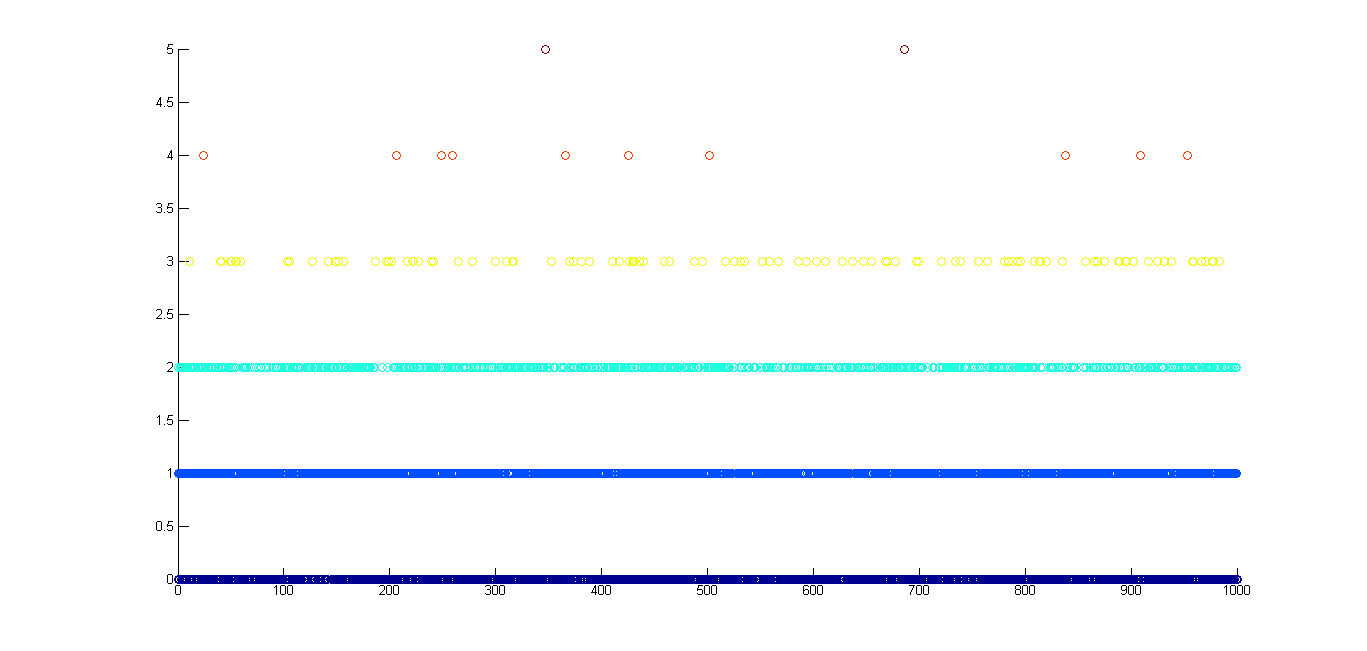
\includegraphics[scale=0.5]{cos1000}
    \caption{Nombre d'ulp d'erreur en fonction de x, pour cos(x)}
    \label{fig:my_label}
\end{figure}

\\
\\
\begin{figure}[h!]
    \centering
    \hspace{-5cm}
    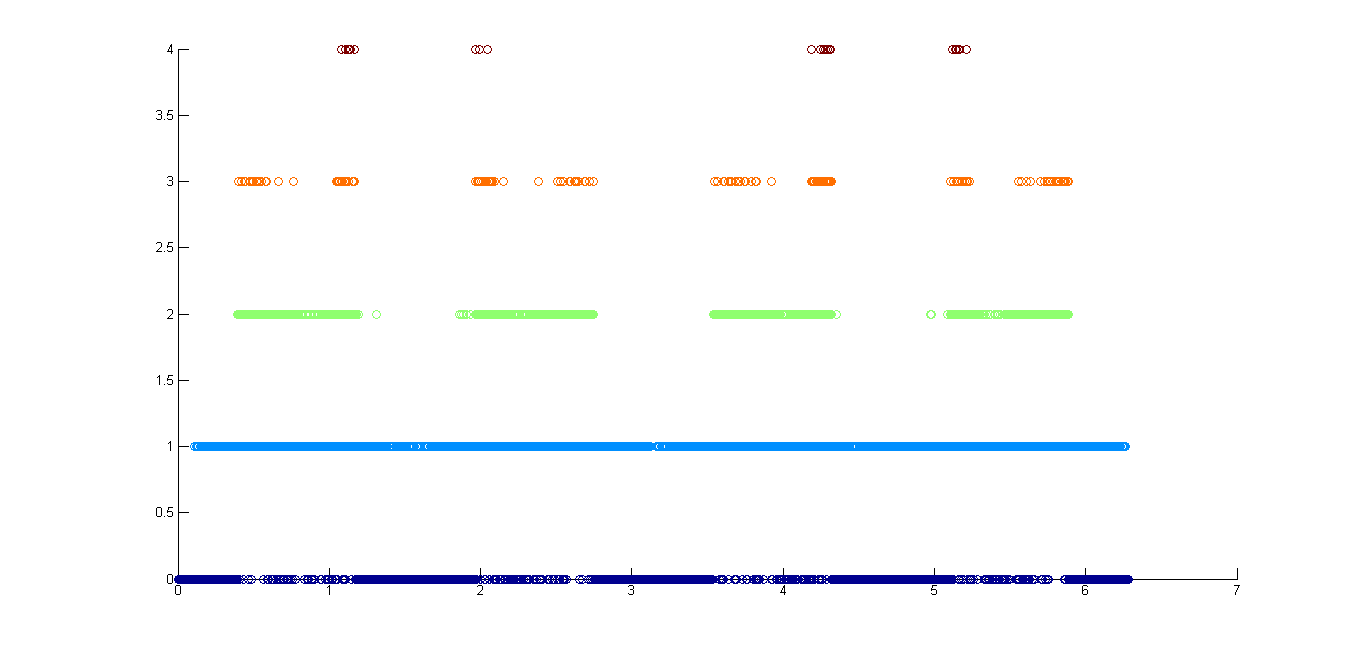
\includegraphics[scale=0.5]{cos2PI}
    \caption{Nombre d'ulp d'erreur en fonction de x, pour cos(x)}
    \label{fig:my_label}
\end{figure}

\\

\cleardoublepage
\section{Fonction atan.}
\subsection{Utilisation des polynômes de Hermite\footnote{http://myweb.lmu.edu/hmedina/papers/arctan.pdf}}
\subsubsection{Justification}
La fonction $arctan$ est facile à décrire avec un développement en série entière mais contrairement aux fonctions $cos$, $sin$, $arcsin$ implémentées, la suite des termes de la série ne convergent pas aussi vite car les coefficients ne comportent pas de termes en factoriels aux dénominateurs.Ceci s'amplifie dès que x s'approche de 1 en valeur absolue.
Les polynômes de hermite sont une meilleure solution.
Ils sont définies par la formule de récurrence suivante: 
$$
p_{1}(x)=4-4x^{2}+5x^{4}-4x^{5}+x^{6}\\
p_{m}(x)=(1-x)^{4}x^{4}p_{m-1}(x)+(-4)^{m-1}p_{1}(x)
$$
\\
On arrive à trouver l'encadrement suivant de la fonction $arctan$ par les polynômes de Hermite:
$$
\mid\int_{0}^{x} (-1)^{m+1}p_{m}(t) \, \mathrm dt - arctan(x))\mid \leq (\frac{1}{4})^{5m}
$$

\\
On montre facilement par récurrence que le polynôme de hermite d'ordre m  est de degré $8m-1$ donc on peut réécrire l'inégalité sous la forme suivante:
$$
\mid\int_{0}^{x} (-1)^{m+1}p_{m}(t) \, \mathrm dt - arctan(x))\mid \leq (\frac{1}{4^{\frac{5}{8}}})^{degr\acute e\ de\ p_{m+1}}
$$
Pour donner un ordre de grandeur le polynôme d'ordre 2 permet une précision de $(\frac{1}{4^{\frac{5}{8}}})^{16}$ =$9.5367431640625.10^-7$ alors que en utilisant un développement en série entière, on doit utiliser un polynôme de degré 1001 pour avoir une précision à 3 décimales près.

\subsubsection{Implémentation}
L'imparité de la fonction arctan nous permet de ramener la résolution sur $\mathds{R}_{+}$\\
Nous avons utilisé les polynômes de Hermite à l'ordre 7 pour nos calculs proche de 0 car la convergence est plus rapide pour des termes proches de 0.
Dans le calcul on a préféré sommer les petits termes en premiers pour imiter l'implémentation de Cody \& Waite.
Si $\mid x \mid$ $>$ 0.6875  et $\mid x \mid$ $<$ 1.1875  nous utilisons la formule trigonométrique suivante pour se ramener à des calculs proche de 0:
$$
{\arctan}~x+{\arctan}~y={\arctan}\left(\frac{x+y}{1-xy}\right)\ avec y=1
$$
Si $\mid x > 1.1875 \mid$ nous utilisons la formule trigonométrique suivante pour se ramener à des termes proches de 0:
$$
\ {\arctan}\ \frac1x+{\arctan}\ x=\frac\pi2
$$


\subsection{Résultats}
Notre implémentation de la méthode \textbf{float Math.atan(float f)} correspond donc à nos attentes, puisque l'on ne dépasse jamais plus de 6 ulp d'erreur.\\
\\

\hspace{-4cm}
\begin{tabular}{|c|c|c|c|c|c|c|}

\hline 
 & intervalle & nombre d'erreur($ > 1 ulp$) & erreur moyenne & erreur max(ulp) & pas & nombres de tests \\
\hline 
arctan & $[0;0.5]$ & 0 & $1$ & 0 &$2^{-17}$ & 65536\\
\hline
arctan & $[0.5;0.72]$ & 224 & 2 &$2$ & $2^{-17}$ & 28836\\
\hline
arctan & $[0.72;0.98]$ & 2888 & 2.12 &$4$ & $2^{-17}$ & 34079\\
\hline
arctan & $[0.98;1]$ & 216 & 2.42 &$6$ & $2^{-17}$ & 2622\\
\hline
\end{tabular}
\\
\\


\begin{figure}[h!]
    \centering
    \hspace{-5cm}
    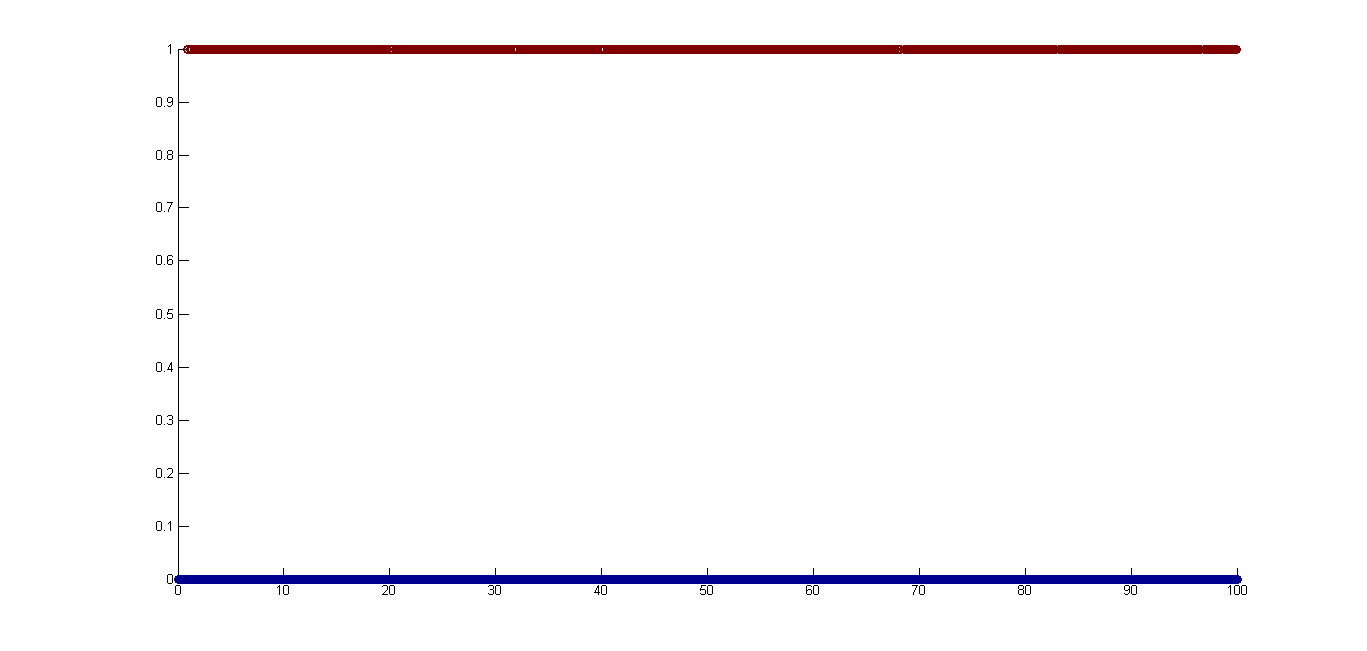
\includegraphics[scale=0.5]{atan100}
    \caption{Nombre d'ulp d'erreur en fonction de x, pour atan(x)}
    \label{fig:my_label}
\end{figure}

\clearpage
\section{Fonction asin.}
\subsection{Utilisation du dévelopement en série entière et de Horner}
Pour le calcul de asin nous avons utilisé la formule classique du développement en série entière de arcsin:
$$
    \sum_{n=0}^{+ \infty}\frac{(2n)!}{(n!2^n)^2} \times \frac{x^{2n+1}}{2n+1} 
$$
La méthode de Horner permet de diminuer le nombre d'opérations en comparaison au calcul de manière basique ce qui améliore la précision de la fonction:
$$a_{n}x^n + . . . + a_{1}x + a_0 = ((. . .(a_{n}x + a_{n-1})x + a_{n-2}). . .) x + a_0$$
Pour un polynôme de degré n ça nous permet de passer de 2n-1 multiplications et n additions à n multiplications et n additions.\\
Si $\mid x \mid< 0.72$ nous utilisons la méthode de horner sur le développement en série entière calculé à l'ordre 33.\\
Si $\mid x \mid> 0.72$ nous utilisons une formule trigonométrique pour se ramener proche de 0:
$$
arcsin(x) = \frac{\pi }{2} - arcsin(\sqrt(1-x^2)) 
$$



\subsubsection{Validation}
La méthode asin donne une approximation à 4 ulp d'écart au maximum.\\
\\

\hspace{-3cm}
\begin{tabular}{|c|c|c|c|c|c|c|}
\hline
 & intervalle & nb erreur($>1 ulp$) & erreur moyenne & erreur max(ulp) & pas & nb tests \\
\hline
asin & $[0;0.5]$ & 0 & 0 & 1 &$2^{-20}$ & 524288\\
\hline
asin & $[0.5;0.72]$ & 1974 & 2 & 2 & $2^{-20}$ & 230687\\
\hline
asin & $[0.72;0.98]$ & 22660 & 2.12 & 4 & $2^{-20}$ & 272630\\
\hline
asin & $[0.98;1]$ & 1687 & 2.43 & 7 & $2^{-20}$ & 20972\\
\hline
\end{tabular}\\
\\

\begin{figure}[h!]
    \centering
    \hspace{-5cm}
    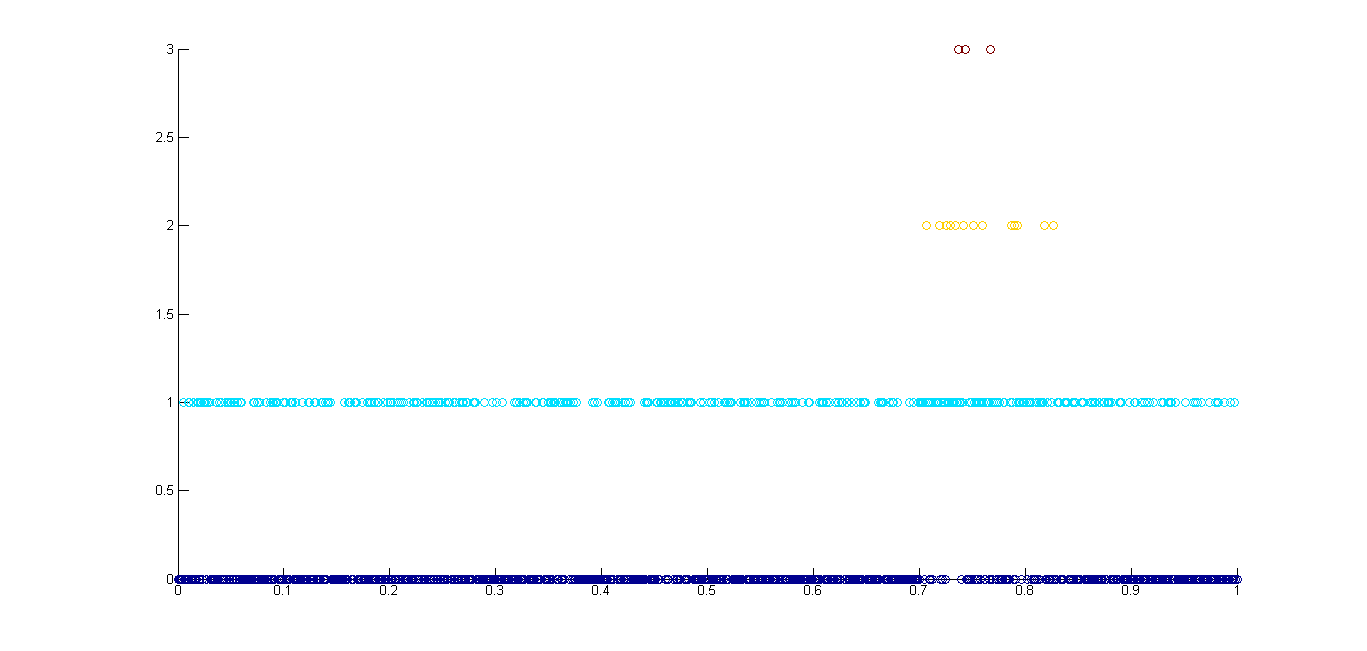
\includegraphics[scale=0.5]{asin}
    \caption{Nombre d'ulp d'erreur en fonction de x, pour asin(x)}
    \label{fig:my_label}
\end{figure}

\end{document}